\FloatBarrier
\chapter{Implementation of machine learning approach in clock bias prediction}


%==================================================================================================
\FloatBarrier
\section{Experimentation environment}

%--------------------------------------------------------------------------------------------------
\FloatBarrier
\subsection{Simulation versus physical environment}

%--------------------------------------------------------------------------------------------------
\FloatBarrier
\subsection{OpenAI Gym}

%--------------------------------------------------------------------------------------------------
\FloatBarrier
\subsection{Selected environments}
Environments selected for use 

\FloatBarrier
\subsubsection{Cart pole}
A pole is attached by a non actuated joint to a cart, which moves along a frictionless track.
The system is controlled by applying a force of +1 or -1 to the cart.
The pendulum starts upright, and the goal is to prevent it from falling over. 
\begin{figure}[htb] 
	\centering
	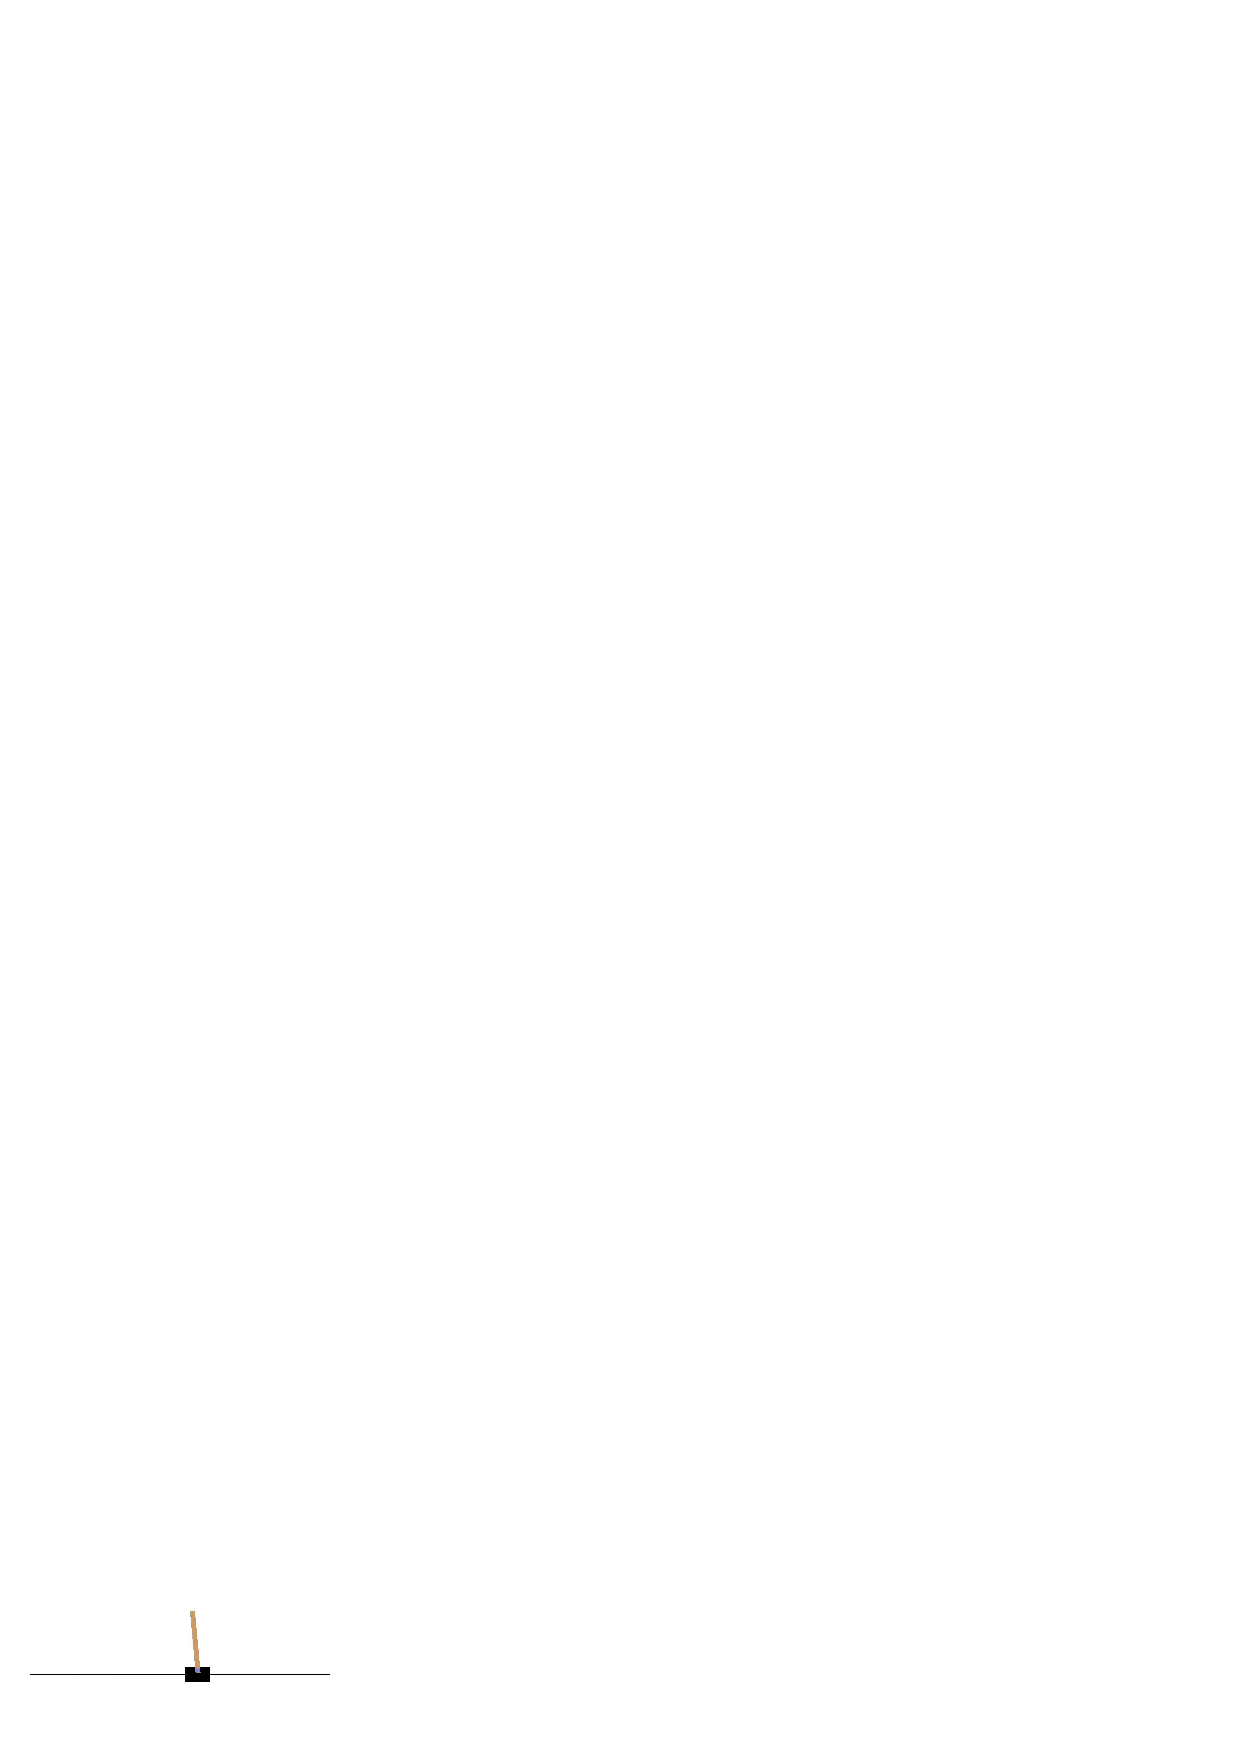
\includegraphics[width=0.6\textwidth]{figures/cartpole}
	\caption{A visualisation of cart pole environment.}
	\label{fig:cartpole}
\end{figure}
A reward of +1 is provided for every cycle that the pole remains upright.
The episode ends when the pole is more than 15 degrees from vertical, or the cart moves more 
than 2.4 units from the center.

\FloatBarrier
\subsubsection{Bipedal walker}
Reward is given for moving forward, total 300 points up to the far end. 
If the robot falls, it gets -100. Applying motor torque costs a small amount of points, 
more optimal agent will get better score.
State consists of hull angle speed, angular velocity, horizontal speed, vertical speed,
position of joints and joints angular speed, legs contact with ground, and 10 lidar 
rangefinder measurements
\begin{figure}[htb] 
	\centering
	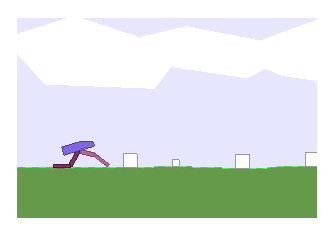
\includegraphics[width=0.6\textwidth]{figures/walker}
	\caption{A visualisation of walker environment in hardcore mode.}
	\label{fig:walker}
\end{figure}
Hardcore version adds ladders, stumps, pitfalls. Time limit is increased due to obstacles. 

\FloatBarrier
\subsubsection{Lunar lander}
Landing pad is always at coordinates (0,0). Coordinates are the first two numbers in state vector.
Reward for moving from the top of the screen to landing pad and zero speed 
is about 100..140 points.
If lander moves away from landing pad it loses reward back. Episode finishes if the lander 
crashes or comes to rest, receiving additional -100 or +100 points.
Each leg ground contact is +10. Firing main engine is -0.3 points each frame.
\begin{figure}[htb] 
	\centering
	
\includegraphics[width=0.6\textwidth]{figures/lunar}
	\caption{A visualisation of lunar lander environment.}
	\label{fig:lunar}
\end{figure}
Solved is 200 points. Landing outside landing pad is possible.
Fuel is infinite, so an agent can learn to fly and then land on its first attempt. 
Action is two real values vector from -1 to +1. First controls main engine, -1..0 off, 0..+1
throttle from 50\% to 100\% power. Engine can't work with less than 50\% power. 
Second value -1.0..-0.5 fire left engine, +0.5..+1.0 fire right engine, -0.5..0.5 off.

\FloatBarrier
\subsubsection{Robotank}
In this environment, the observation is an RGB image of the screen, which is an array of shape 
(210, 160, 3).

In Robotank, player is in control of a tank located in the middle of a barren field and must 
destroy enemy tanks after pinpointing their positions by using the window view and a small 
radar scope.

As shown on Figure \ref{fig:robotank}, game display is divided into two sections. 
The majority of the screen is occupied by the view of the battlefield, only objects in 
the front of vechicle are visible. 
The remainder of the screen consists of the status panel.

Located in the center of the status panel is a circular radar display with a sweeping arm.
If there is an enemy tank on the battlefield, it will appear on this display as a pink dot 
relative to robot position.
\begin{figure}[htb] 
	\centering
	\includegraphics[width=\textwidth]{figures/robotank}
	\caption{A visualisation of robotank game frame that also serves as an input for network.}
	\label{fig:robotank}
\end{figure}

Situated around the radar display are four yellow boxes with capital letters in them.
These are the damage indicators. When your tank is shot, you suffer either a direct hit or a 
glancing shot. The first destroys your tank, the latter merely damages it.
The type of damage inflicted upon your tank is random.
If the V box is on, your video display will flash on and off. C means that your cannon 
firing power is cut in half. R indicates that your radar has been rendered useless.
T simply slows down the turning ability of your Robotank

%==================================================================================================
\FloatBarrier
\section{Topological neural network implementation in low resource environment}

%--------------------------------------------------------------------------------------------------
\FloatBarrier
\subsection{Native implementation on 64-bit architecture}

%--------------------------------------------------------------------------------------------------
\FloatBarrier
\subsection{Limitations in used embedded system}

%--------------------------------------------------------------------------------------------------
\FloatBarrier
\subsection{Computation efficiency - 24-bit fixed point model}

%--------------------------------------------------------------------------------------------------
\FloatBarrier
\subsection{Memory efficiency - offset based model}
